

Consider the linear optimization problem
\[
\min_{x \in \R^2} x_1
\]
subject to
\[
x_1, x_2 \geq 0.
\]
For any $\alpha \geq 0$, the solution
\[
\cvect{0 \\ \alpha}
\]
is optimal. Indeed, it is feasible, and $x_1$ achieves its smallest
possible value. Therefore, the problem has an inifinite number of
optimal solutions. 
The feasible set is the non negative quadrant. It has only one vertex:
\[
\cvect{0 \\ 0},
\]
as illustrated in the following figure: 
\begin{center}
  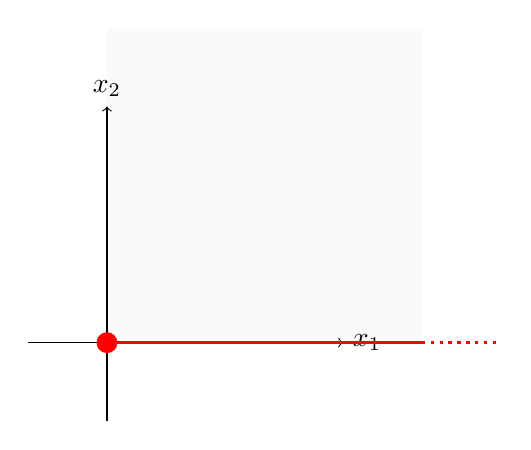
\begin{tikzpicture}
  \fill[gray!20,opacity=0.2] (0,0) rectangle (4,4) ;
  %\draw[fill=gray!50,opacity=0.2] (0,0)--(4,0)--(4,4)--(0,4)--cycle;
  \draw[->] (-1,0) -- (3,0) node[right] {$x_1$};
  \draw[->] (0,-1) -- (0,3) node[above] {$x_2$};
  
  \node [circle,fill=red,scale=0.8] at (0,0){};
  \draw[very thick,red] (0,0)--(4,0);
  \draw[very thick,red,style=dotted] (4,0)--(5,0);
  
\end{tikzpicture}
\end{center}
Consequently, the claim is not true. 

